\exo{6}{Représenter}

Effectuer les transformations suivantes.

\begin{minipage}[t]{0.45\textwidth} 
    La symétrie axiale d'axe $(d)$
    \begin{figure}[H]
        \centering
        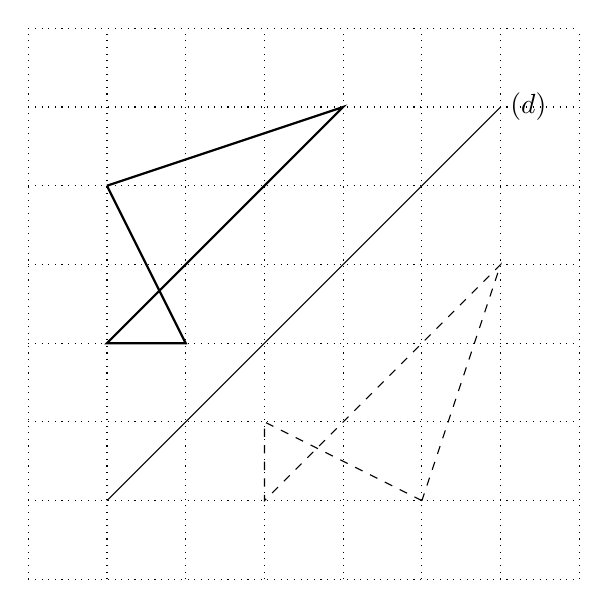
\begin{tikzpicture}[scale=1]
            \def\mypath{(-2,2) -- (-1,0) --(-2,0) -- (1,3)--(-2,2)}
            \draw [thick]\mypath ;
            \draw (-2,-2)--(3,3) node [right]{$(d)$} ;
            \draw [cm={0,1,1,0,(0,0)},dashed] \mypath;%Matrice de transformation inverse X et Y
            \draw [dotted](-3,-3) grid (4,4);
        \end{tikzpicture}
    \end{figure}
\end{minipage}
\hfill
\begin{minipage}[t]{0.45\textwidth}
    La translation qui amène $A$ sur $B$
    \begin{figure}[H]
        \centering
        \begin{tikzpicture}[scale=1]
            \def\mypath{(-2,-2) -- (-1,1) --(-2,0) -- (-1,2)--(0,-2)--(-2,-2)}
            \draw [thick]\mypath ;
            \fill (1,-1) coordinate (c) circle(2pt) node[above] {$A$};            
            \fill (4,1) coordinate (c) circle(2pt) node [above]{$B$};    
            \draw[dashed,shift=(3,2)]\mypath  ;      
            \draw [dotted](-3,-3) grid (4,4);
        \end{tikzpicture}
    \end{figure}
\end{minipage}

\begin{minipage}[t]{0.45\textwidth} 
    La symétrie centrale de centre $O$
    \begin{figure}[H]
        \centering
        \begin{tikzpicture}[scale=1]
            \tikzset{
            homothety at/.style args={#1 scaled by #2}{shift={($(#1)!#2!(0,0)$)},scale=#2},}
            \def\mypath{(-2,2) -- (-1,0) --(-2,0) -- (1,3)--(-2,2)}
            \draw [thick]\mypath ;
            \fill (0,0) coordinate (c) circle(2pt) node [above]{$O$};     
            \begin{scope}[homothety at=c scaled by -1]
                \draw[dashed] \mypath;
            \end{scope}        
            \draw [dotted](-3,-3) grid (4,4);
        \end{tikzpicture}
    \end{figure}
\end{minipage}
\hfill
\begin{minipage}[t]{0.45\textwidth}
    L'homothétie de centre $O$ et de rapport -2.
    \begin{figure}[H]
        \centering
        \begin{tikzpicture}[scale=1]
            \tikzset{
            homothety at/.style args={#1 scaled by #2}{shift={($(#1)!#2!(0,0)$)},scale=#2},}
            \def\mypath{(-2,-2) -- (-1,1) --(-2,0) -- (-1,0)--(0,-2)--(-2,-2)}
            \draw [thick]\mypath ;
            \fill (0,0) coordinate (c) circle(2pt) node [above]{$O$};     
            \begin{scope}[homothety at=c scaled by -2]
                \draw[dashed] \mypath;
            \end{scope}        
            \draw [dotted](-3,-3) grid (4,4);
        \end{tikzpicture}
    \end{figure}
\end{minipage}

\begin{minipage}[t]{0.45\textwidth} 
    L'homothétie de centre $O$ et de rapport -0.5
    \begin{figure}[H]
        \centering
        \begin{tikzpicture}[scale=1]
            \tikzset{
            homothety at/.style args={#1 scaled by #2}{shift={($(#1)!#2!(0,0)$)},scale=#2},}
            \draw [white](-3,-4) grid (4,3);
            \def\mypath{(0,0) -- (-2,3) --(-2,0) -- (-1,-4)--(0,0)}
            \draw [thick]\mypath ;
            \fill (2,0) coordinate (c) circle(2pt) node [above]{$O$};     
            \begin{scope}[homothety at=c scaled by -0.5]
                \draw[dashed] \mypath;
            \end{scope}        
        \end{tikzpicture}
    \end{figure}
\end{minipage}
\hfill
\begin{minipage}[t]{0.45\textwidth}
    L'homothétie de centre $O$ et de rapport 2.
    \begin{figure}[H]
        \centering
        \begin{tikzpicture}[scale=1]
            \tikzset{
            homothety at/.style args={#1 scaled by #2}{shift={($(#1)!#2!(0,0)$)},scale=#2},}
            \draw [white](-3,-3) grid (4,4);
            \def\mypath{(-2,-2) -- (-1,1) -- (-1,0)--(1,-2)--(-2,-2)}
            \draw [thick]\mypath ;
            \fill (-3,0) coordinate (c) circle(2pt) node [above]{$O$};     
            \begin{scope}[homothety at=c scaled by 2]
                \draw[dashed] \mypath;
            \end{scope}        
        \end{tikzpicture}
    \end{figure}
\end{minipage}

\exo{4}{Raisonner}

Trouver le centre de chacune des homothéties suivantes.

\begin{minipage}[t]{0.45\textwidth}  
    \begin{figure}[H]
        \centering
		\begin{tikzpicture}[scale=0.8]
            \tikzset{
            homothety at/.style args={#1 scaled by #2}{shift={($(#1)!#2!(0,0)$)},scale=#2},}
            \def\mypath{(8,0)--(0,0)--(0,8)--(8,8)}
            \draw [white](0,0) grid (8,8);
            \draw [thick]\mypath ;
            \fill (4.7,5.7) coordinate (c) circle(2pt);
            \begin{scope}[homothety at=c scaled by -0.6]
                \draw[dashed] \mypath;
            \end{scope}
        \end{tikzpicture}
    \end{figure}
\end{minipage}
\hfill
\begin{minipage}[t]{0.45\textwidth}  
    \begin{figure}[H]
        \centering
        \begin{tikzpicture}[scale=0.8]
            \tikzset{
            homothety at/.style args={#1 scaled by #2}{shift={($(#1)!#2!(0,0)$)},scale=#2},}
            \def\mypath{(7,0)--(4,1)--(4,0)--(0,0)--(0,3)--(4,1)}
            \draw [white](0,0) grid (8,8);
            \draw [thick]\mypath ;
            \fill (8,8) coordinate (c) circle(2pt);
            \begin{scope}[homothety at=c scaled by 0.7]
                \draw[dashed] \mypath;
            \end{scope}
        \end{tikzpicture}
    \end{figure}
\end{minipage}

\begin{minipage}[t]{0.45\textwidth}  
    \begin{figure}[H]
        \centering
        \begin{tikzpicture}[scale=0.8]
            \tikzset{
            homothety at/.style args={#1 scaled by #2}{shift={($(#1)!#2!(0,0)$)},scale=#2},}
            \def\mypath{(2,0)--(2,3)--(3,4)--(2,0)}
            \draw [white](0,0) grid (8,8);
            \draw [thick]\mypath ;
            \fill (0,0) coordinate (c) circle(2pt);
            \begin{scope}[homothety at=c scaled by 2]
                \draw[dashed] \mypath;
            \end{scope}
        \end{tikzpicture}
    \end{figure}
\end{minipage}
\hfill
\begin{minipage}[t]{0.45\textwidth}  
    \begin{figure}[H]
        \centering
        \begin{tikzpicture}[scale=0.8]
            \tikzset{
            homothety at/.style args={#1 scaled by #2}{shift={($(#1)!#2!(0,0)$)},scale=#2},}
            \def\mypath{(2,2)--(2,4)--(3,4)--(4,4)--(3,2)--(2,2)}
            \draw [white](0,0) grid (8,8);
            \draw [thick]\mypath ;
            \fill (5,1) coordinate (c) circle(2pt);
            \begin{scope}[homothety at=c scaled by 1.7]
                \draw[dashed] \mypath;
            \end{scope}
        \end{tikzpicture}
    \end{figure}
\end{minipage}